\section{Statistiken von Funktionsargumenten}
\label{args_stat}

Ich war immer sehr daran interessiert welches die durchschnittliche Anzahl von
Argumenten der einzelnen Funktionen ist.

\index{UNIX!grep}
Dazu wurden viele Windows 7 32-Bit-DLLs analysiert
(crypt32.dll, mfc71.dll, msvcr100.dll, shell32.dll, user32.dll, d3d11.dll, mshtml.dll,
msxml6.dll, sqlncli11.dll, wininet.dll, mfc120.dll, msvbvm60.dll, ole32.dll, themeui.dll,
wmp.dll), da diese die stdcall-Konvention nutzen, was es einfach macht das Ergebnis des
Disassemblers mit grep nach \INS{RETN X} zu durchsuchen.

\begin{itemize}
\item keine Argumente: ~29\%
\item 1 Argument: ~23\%
\item 2 Argumente: ~20\%
\item 3 Argumente: ~11\%
\item 4 Argumente: ~7\%
\item 5 Argumente: ~3\%
\item 6 Argumente: ~2\%
\item 7 Argumente: ~1\%
\end{itemize}

\begin{figure}[H]
\centering
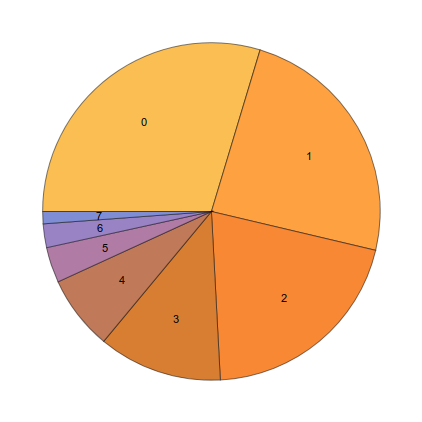
\includegraphics[width=0.5\textwidth]{other/args_stat.png}
\caption{Statistiken von Funktionsargumenten}
\end{figure}

Das Ergebnis ist stark vom Programmierstil abhängig und kann bei anderen Programmen
deutlich anders ausfallen.
